\documentclass{standalone}
\usepackage{tikz}
\usetikzlibrary{patterns}

\begin{document}
    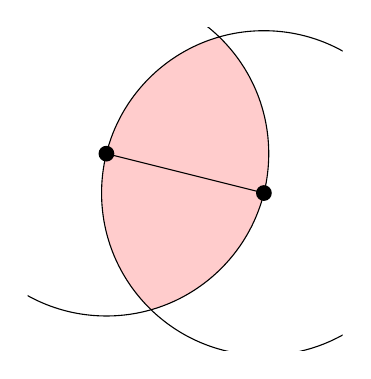
\begin{tikzpicture}
        \clip (-2,2.1) rectangle (2,-2);
        % Shade the intersection where signals collide.
        \begin{scope}
            \clip (-1, 0.5) circle(2.06155281281);
            \fill[fill=red!20] (1, 0) circle(2.06155281281);
        \end{scope}

        \draw (-1, 0.5) circle(2.06155281281);
        \fill (-1, 0.5) circle(0.1);
        \draw (1, 0) circle(2.06155281281);
        \fill (1, 0) circle(0.1);
        \draw (1, 0) -- (-1, 0.5);
    \end{tikzpicture}
\end{document}
